\documentclass[11pt, titlepage,a4paper]{article}
\usepackage[utf8]{inputenc}
\usepackage[square,sort,comma,numbers]{natbib}
\usepackage{hyperref}
\usepackage{dsfont}
\usepackage{subfigure}
\usepackage{multicol}
\usepackage[T1]{fontenc}
\usepackage[left=2cm,right=2cm,top=2cm,bottom=2cm]{geometry}
\usepackage[spanish, activeacute]{babel}
\usepackage{amsmath}
\usepackage{amssymb,amsfonts,textcomp}
\usepackage{color}
\usepackage{array}
\usepackage{hhline}
\usepackage{varwidth}
\usepackage{graphicx}
\usepackage{parcolumns}
%\usepackage{cite}
\usepackage{hyperref}
\usepackage[]{algorithm2e}


\hypersetup{ colorlinks=true, linkcolor=black, citecolor=black, filecolor=black,
urlcolor=blue, pdftitle=Laboratorio 6: Clustering Jerarquico , pdfauthor= Alberto Fernández Arkaitz Marcos Endika Serrano}

\bibliographystyle{plain}


\renewcommand{\thefootnote}{\fnsymbol{footnote}}
\title{\textbf{\huge{Mineria de Datos} \\Laboratorio 6: Clustering
Jerarquico \newline
\begin{center}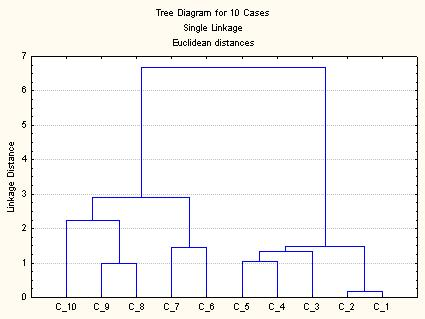
\includegraphics[scale =
1.4]{./images/Portada.jpg}\newline\footnote{Imagen extraida de
\url{http://jmj-qa.blogspot.com.es/2011/09/analisis-cluster.html}}\end{center}}
}


\author{Alberto Fernández \and Arkaitz Marcos \and Endika Serrano}
\date{}

\begin{document}
\maketitle

\tableofcontents

\newpage
\renewcommand{\thefootnote}{\arabic{footnote}}

\section{Introducción}

El objetivo de esta práctica es la programación de un algoritmo de clustering
jerárquico evitando la utilización de librerías de terceros y tratando de
mejorar el rendimiento frente a programas de minería de datos de uso general
como puede ser \textbf{Weka}.


\subsection{Definición}
 
\paragraph{Clasificación no-supervisada:\\}
Los métodos de clasificación en los que los datos de entrenamiento son vectores
x sin una clase definida.\cite[Página 3, 2º Párrafo]{Bishop} 


La clasificación no supervisada tiene como objetivo la agrupación de datos en
grupos, estas agrupaciones tienen valor por sí mismas y su clasificación no
tiene interés.para ello emplea la similitud/disimilitud entre los atributos de
las distintas instancias para poder realizar la “clasificación� sin contar con
la clase definida que le indique la clasificación correcta o el grado de error
en las distintas predicciones.\cite[Página 486,3ºlinea]{Elements}  
\cite[Sección 14.1, 1º Párrafo]{Handbook}


\subsection{Objetivo}
El objetivo de esta práctica es el diseño e implementación de un algoritmo de
clasificación no supervisada mediante la técnica del Clustering Jerárquico,
tanto en su variante  como Aglomerativa como Divisiva evitando la utilización de
librerías de terceros.
\bigskip
Hemos utilizado principalmente los siguientes archivos:
%
\begin{description}
\item[color.arff]Este fichero cuenta con 62 instancias y 2001 atributos
numéricos junto con la clase nominal.
\item[food.arff]Este fichero cuenta con 24 instancias y 6 atributos, de los
cuales 5 son numéricos y 1 de tipo string.
\end{description}

\section{Algoritmo}
\subsection{Aglomerativo}
\begin{center}
\fbox{%
\begin{varwidth}{\dimexpr\linewidth-2\fboxsep-2\fboxrule\relax}
\begin{enumerate}
\item iteration $\leftarrow$ 1 
\item while \{iteration < nº Instancias\}

\subitem merge the best 2 clusters (the nearest) and add it in the cluster
list after removing the merged clusters

\subitem create a new Iteration including the new cluster list

\subitem add the new Iteration to the last position of the list of
iterations

\item do iteration $\leftarrow$ iteration +1 

\end{enumerate}
	\end{varwidth}% 
		
	}
\end{center}
%Clustering jerarquico en pseudocodigo

\subsection{Divisivo}
\begin{center}

\fbox{%
\begin{varwidth}{\dimexpr\linewidth-2\fboxsep-2\fboxrule\relax}
\begin{enumerate}
\item iteration $\leftarrow$ 1 
\item while \{iteration < nº Instancias\}

\subitem divide the best clusters (the furthest instances in the cluster) and
add the new cluster to the cluster list

\subitem create a new Iteration including the new cluster list

\subitem add the new Iteration to the last position of the list of
iterations

\item do iteration $\leftarrow$ iteration +1 

\end{enumerate}
	\end{varwidth}% 
		
	}
\end{center}

\section{Diseño}
\begin{figure}[hbtp]
\centering
\includegraphics[scale = 0.18]{images/DiagramaP}
\end{figure}

\subsection{packIO}
En este paquete se agrupan las clases cuya funcionalidad principal es la entrada
y salida de datos.

\subsubsection{Loader}
Esta clase se encarga de cargar en la aplicación los datos contenidos en los
ficheros \textit{arff}.

\subsubsection{Printer}
Esta clase es la encargada de representar los datos. Sus principales
funcionalidades son la salida por pantalla de los resultados obtenidos, la
creación de un dendograma que represente los datos, y la salida a ficheros de
esos datos como txt y pdf.

\subsection{packDistancias}
\label{packDistancias}
En este paquete se agrupan las clases cuya funcionalidad principal es el calculo
de distancias entre instancias.

\subsubsection{Metrica}
Esta clase es la encargada de realizar los cálculos de distancias entre
instancias utilizando distintas métricas:
\begin{itemize}
  \item Euclidea
  \item Manhattan
  \item Minkowski
\end{itemize}

\subsubsection{Distancia}
Esta clase es la encargada de realizar los cálculos de distancias en conjunto
con la clase Metrica utilizando distintas métricas:
\begin{itemize}
  \item Complete
  \item Simple
  \item Average
\end{itemize}

\subsection{packJerarquico}
En este paquete se agrupan las clases cuya función es la ejecución de los
algoritmos de clustering jerárquico y las clases necesarias para almacenar las
estructuras generadas por los mismos.

\subsubsection{Main}
Es la clase encargada de capturar los argumentos necesarios para la ejecución
del programa y una vez recogidos lanzar el proceso.
 
\subsubsection{ListofIterations}
Esta clase es la encargada de guardar las iteraciones generadas durante la
ejecución del algoritmo de clustering. Ademas es la clase que realiza el
clustering en sus variantes:
\begin{itemize}
  \item Aglomerativo
  \item Divisivo
\end{itemize}

\subsubsection{Iteration}
Esta clase es la encargada de guardar la lista de clusters que hay durante la
iteración así como el nombre de la iteración y una lista con las distancias
entre los clusters de la lista anterior.

Es la encargada de generar nuevos clusters e incluirlos en una nueva iteración,
tanto uniendo dos clusters como dividiendo uno.

\subsubsection{Cluster}
Esta clase almacena el numero (nombre) del cluster, las instancias que lo forman,
su centroide, la iteración en la que se ha creado así como los clusters a partir
del cual se ha generado.

\subsubsection{Distance}
Esta clase almacena la distancia entre dos clusters así como los clusters entre
los cuales se calculado la distancia.

Es también la encargada de calcular la distancia llamando a las clases
contenidas en el
\ref{packDistancias}\textit{packDistancias}\ref{packDistancias}.

\subsubsection{ListOfInstances}
Es la clase encargada de almacenar las distintas instancias que se van a
utilizar en la aplicación.

\subsubsection{Instances}
Es la clase que almacena el nombre de cada instancia y los atributos que la
forman, esta aplicación solamente soporta atributos numéricos, por lo que
solamente se almacenan atributos numéricos.


\section{Resultados experimentales}

\subsection{Banco de pruebas}
Para realizar las pruebas hemos empleado la versión final de la aplicación y el
fichero food.arff. hemos empleado tanto la versión aglomerativa como la divisiva
del algoritmo en todas las variantes de métrica(Euclidean, Minkoswki, Manhattan)
y cálculo de distancia(Simple, Complete, Average) empleando para Minkowski k = 7


\subsection{Resultados obtenidos}
\paragraph{Clustering Aglomerativo\\}
\begin{itemize}
  \item Simple
  	\subitem Euclidean
  		\subsubitem Tiempo: 2s
  		\subsubitem Fichero de resultados: food.arff1413735972118.pdf
	\subitem Manhattan
		\subsubitem Tiempo: 2s
  		\subsubitem Fichero de resultados: food.arff1413736110243.pdf
	\subitem Minkowski k = 7
		\subsubitem Tiempo: 3s 
  		\subsubitem Fichero de resultados: food.arff1413736304808.pdf 	
  \item Complete
	\subitem Euclidean
  		\subsubitem Tiempo: 2s
  		\subsubitem Fichero de resultados: food.arff1413736445797.pdf 
	\subitem Manhattan
		\subsubitem Tiempo: 2s
  		\subsubitem Fichero de resultados: food.arff1413736535402.pdf 
	\subitem Minkowski k = 7
		\subsubitem Tiempo: 2s
  		\subsubitem Fichero de resultados: food.arff1413736641739.pdf 	
  \item Average
  	\subitem Euclidean
  		\subsubitem Tiempo: 2s
  		\subsubitem Fichero de resultados: food.arff1413736708556.pdf 
	\subitem Manhattan
		\subsubitem Tiempo: 2s
  		\subsubitem Fichero de resultados: food.arff1413736777966.pdf
	\subitem Minkowski k = 7
		\subsubitem Tiempo: 2s
  		\subsubitem Fichero de resultados: food.arff1413736821139.pdf	
\end{itemize}

\paragraph{Clustering Divisivo\\}
\begin{itemize}
  \item Simple
  	\subitem Euclidean
  		\subsubitem Tiempo: 2s
  		\subsubitem Fichero de resultados: food.arff1413738583516.pdf
	\subitem Manhattan
		\subsubitem Tiempo: 2s
  		\subsubitem Fichero de resultados: food.arff1413738547888.pdf
	\subitem Minkowski k = 7
		\subsubitem Tiempo: 2s
  		\subsubitem Fichero de resultados: food.arff1413738467626.pdf	
  \item Complete
	\subitem Euclidean
  		\subsubitem Tiempo: 2s
  		\subsubitem Fichero de resultados: food.arff1413738635058.pdf
	\subitem Manhattan
		\subsubitem Tiempo: 2s
  		\subsubitem Fichero de resultados: food.arff1413738739824.pdf
	\subitem Minkowski k = 7
		\subsubitem Tiempo: 2s
  		\subsubitem Fichero de resultados: food.arff1413738769585.pdf
  \item Average
  	\subitem Euclidean
  		\subsubitem Tiempo: 2s
  		\subsubitem Fichero de resultados: food.arff1413738084408.pdf
	\subitem Manhattan
		\subsubitem Tiempo: 2s
  		\subsubitem Fichero de resultados: food.arff1413738360677.pdf
	\subitem Minkowski k = 7
		\subsubitem Tiempo: 2s
  		\subsubitem Fichero de resultados: food.arff1413738418598.pdf	
\end{itemize}

\subsection{Resultados respecto a otro software}

\subsection{Análisis de resultados}


\subsection{Rendimiento del software}
Con respecto al rendimiento simplemente señalar que la variante aglomerativa
tarda más que la variante divisiva por el mero hecho de que esta última no
genera un dendograma al acabar de ejecutarse.

\section{Conclusiones}
La motivación principal para aplicar técnicas de clustering es agrupar grandes
conjuntos de datos de forma que se cada grupo formado tenga unas características similares y de esta forma sea posible analizar los datos sin un inmenso coste temporal.

Se observa un gran aumento de rendimiento respecto a las aplicaciones con
interfaz gráfica y de uso menos específico (\textit{Weka}). Además el dendograma generado es de menor complejidad y mayor comprensión a pesar de que no indica las distancias de unión.

Uno de los cambios más significativos podría ser el que aceptase archivos
\textit{CSV} para ahorrar tiempo del usuario en convertirlo a \textit{ARFF}.
 
Se podría mejorar el dendograma de forma que aparecieran las distancias de la
unión entre clusters para una mayor comprensión visual. 

Sería interesante mejorar el algoritmo divisivo de forma que aparezca el
dendograma.

\section{Bibliografía}
\renewcommand{\refname}{\ }

\begin{thebibliography}{1}
	
	\bibitem{Bishop}
	{\em Pattern Recognition and Machine Learning}.
	\newblock Springer, 2006.
	
	\bibitem{Elements}
	{\em The Elements of Statistical Learning Data Mining,Inference,and Prediction:
		Second Edition}.
	\newblock Springer, 2009.
	
	\bibitem{Handbook}
	{\em Data Mining and Knowledge Discovery Handbook:Second Edition}.
	\newblock Springer, 2011.
	
	\bibitem{Witten}
	{\em Practical Machine Learning Tools and Techniques}.
	\newblock Morgan Kaufmann, 2011.
	
\end{thebibliography}

\section{Valoración subjetiva}

\subsection{Alberto Fernández}
\paragraph{¿Has alcanzado los objetivos que se plantean?\\}
Sí, creo que he alcanzado los objetivos que se plantean para esta práctica.

\paragraph{¿Te ha resultado de utilidad la tarea planteada?\\}
Esta tarea me ha resultado de utilidad para ver mis capacidades para afrontar
una un problema 'nuevo' de forma más o menos autónoma.

\paragraph{¿Qué dificultades has encontrado? Valora el grado de dificultad de
la tarea\\}
La mayor dificultad con la que me he encontrado ha sido el desconocimiento sobre
este tipo de problemas y la improvisación a la que me ha llevado dicho desconocimiento.

\paragraph{¿Cuánto tiempo has trabajado en esta tarea? Desglosado:\\}
\begin{description}
	\item[Tiempo de diseño de software] 2h
	\item[Tiempo de implementación de software] 26h
	\item[Tiempo trabajando con Weka] 0h
	\item[Tiempo dedicado a búsqueda bibliográfica] 3h
	\item[Tiempo redactando el informe] 10h (problemas durante la edición)
\end{description}

\paragraph{Sugerencias para mejorar la tarea. Sugerencias para que se consiga despertar mayor
interés y motivación en los alumnos.\\}

\paragraph{Críticas (constructivas).\\}
El enunciado de la tarea podría estar desglosado para el algoritmo
\textit{k-means} y \textit{clustering jerárquico} para de esta forma evitar confusiones.

\subsection{Arkaitz Marcos}
\paragraph{¿Has alcanzado los objetivos que se plantean?\\}
Sí, en mi opinión si he logrado alcanzar los objetivos planteados.

\paragraph{¿Te ha resultado de utilidad la tarea planteada?\\}
Sí, ya que me ha ayudado a superar los obstaculos encontrados y la frustación
ante los fallos cometidos.

\paragraph{¿Qué dificultades has encontrado? Valora el grado de dificultad de
la tarea\\}
La primera de las dificultades encontradas ha sido el planteamiento de la
implementación del algoritmo sin utilizar las librerías de weka, aunque también
fue una de las más fáciles de solucionar.
Otra de las dificultades más complicadas ha sido intentar dibujar el dendograma
del algoritmo divisivo el cual finalmente no ha podido desarrollarse.
El grado de dificultad ha sido medio.

\paragraph{¿Cuánto tiempo has trabajado en esta tarea? Desglosado:\\}
\begin{description}
	\item[Tiempo de diseño de software] 1h
	\item[Tiempo de implementación de software] 18h
	\item[Tiempo trabajando con Weka] 0h
	\item[Tiempo dedicado a búsqueda bibliográfica] 0h
	\item[Tiempo redactando el informe] 2h
\end{description}

\paragraph{Sugerencias para mejorar la tarea. Sugerencias para que se consiga despertar mayor
interés y motivación en los alumnos.\\}
La tarea esta bien especificada para su realización y cumplimiento de los
objetivos. Ninguna sugerencia.

\paragraph{Críticas (constructivas).\\}
Estoy de acuerdo con Alberto en cuando al desglose del enunciado de la tarea.

\subsection{Endika Serrano}
\paragraph{¿Has alcanzado los objetivos que se plantean?\\}
Sí, al menos los principales se han alcanzado.
\paragraph{¿Te ha resultado de utilidad la tarea planteada?\\}
Sí, esta práctica nos ha ayudado a aprender a programar sin usar las librerías de Weka y eso nos ha supuesto un reto.
 \paragraph{¿Qué dificultades has encontrado? Valora el grado de dificultad de
la tarea\\}
El empezar algo de cero con total desconocimiento. El grado de dificultad ha
sido alto.
\paragraph{¿Cuánto tiempo has trabajado en esta tarea? Desglosado:\\}
\begin{description}
	\item[Tiempo de diseño de software] 2h
	\item[Tiempo de implementación de software] 8h
	\item[Tiempo trabajando con Weka] 5h
	\item[Tiempo dedicado a búsqueda bibliográfica] 1h
	\item[Tiempo redactando el informe] 1h
\end{description}

\paragraph{Sugerencias para mejorar la tarea. Sugerencias para que se consiga despertar mayor
interés y motivación en los alumnos.\\}

\paragraph{Críticas (constructivas).\\}
Estaría bien que el clustering jerárquico tuviese su propio apartado y no tener
que usar el guion del k-means.
\end{document}